\documentclass[a4paper,12pt,obeyspaces,spaces,hyphens]{article}

\usepackage{agenda}
\usepackage{colortbl}
\usepackage{xcolor}
\usepackage{calc}

\hypersetup{pdftitle={Embedded Linux kernel and driver development training},
  pdfauthor={Bootlin}}

\renewcommand{\arraystretch}{2.0}

\begin{document}

\thispagestyle{fancy}

\setlength{\arrayrulewidth}{0.8pt}

\begin{center}
\LARGE
Embedded Linux kernel and driver development training\\
\large
5-day session
\end{center}
\vspace{1cm}

\small
\newcolumntype{g}{>{\columncolor{fedarkblue}}m{4cm}}
\newcolumntype{h}{>{\columncolor{felightblue}}X}

\arrayrulecolor{lightgray} {
  \setlist[1]{itemsep=-5pt}
  \begin{tabularx}{\textwidth}{|g|h|}
    {\bf Title} & {\bf Embedded Linux kernel and driver development training} \\
    \hline

    {\bf Overview} &
    Understanding the Linux kernel \par
    Developing Linux device drivers \par
    Linux kernel debugging \par
    Porting the Linux kernel to a new board \par
    Working with the kernel development community \par
    Practical labs with the ARM-based BeagleBone Black board
    (or with its Wireless variant).\\
    \hline
    {\bf Materials} &
    Check that the course contents correspond to your needs:
    \newline \url{https://bootlin.com/doc/training/linux-kernel}. \\
    \hline

    {\bf Duration} & {\bf Five} days - 40 hours (8 hours per day).
    \newline 50\% of lectures, 50\% of practical labs. \\
    \hline

    {\bf Trainer} & One of the engineers listed on
    \newline \url{https://bootlin.com/training/trainers/}\\
    \hline

    {\bf Language} & Oral lectures: English or French.
    \newline Materials: English.\\
    \hline

    {\bf Audience} & People developing devices using the Linux kernel
    \newline People supporting embedded Linux system developers. \\
    \hline

    {\bf Prerequisites} &

    {\bf Solid experience in C programming}
    \newline In particular, participants must be familiar
    with creating and dealing with complex data types and structures,
    with pointers to such symbols, as well as with function pointers. \vspace{1em}
    \newline {\bf Knowledge and practice of UNIX or GNU/Linux commands}
    \newline People lacking experience on this topic should get
    trained by themselves, for example with our freely available on-line slides
    (\url{https://bootlin.com/blog/command-line/}).\vspace{1em}
    \newline {\bf Experience in embedded Linux development}.
    \newline Taking our Embedded Linux course
    (\url{https://bootlin.com/training/embedded-linux/})
    first is not an absolute prerequisite, but it will definitely
    help people lacking embedded Linux development experience.
    They will understand the development environment
    and board manipulations better, allowing them to concentrate on
    kernel code programming.
    \\
    \hline
  \end{tabularx}

  \begin{tabularx}{\textwidth}{|g|h|}
    {\bf Required equipment} &
    {\bf For on-site sessions only}
    \newline Everything is supplied by Bootlin in public sessions.
    \begin{itemize}
    \item Video projector
    \item PC computers with at least 8 GB of RAM, and Ubuntu Linux
    installed in a {\bf free partition of at least 20 GB. Using Linux
      in a virtual machine is not supported}, because of issues
    connecting to real hardware.
    \item We need Ubuntu Desktop 20.04 (Xubuntu and
    other variants are fine). We don't support other
    distributions, because we can't test all possible package versions.
    \item {\bf Connection to the Internet} (direct or through the
    company proxy).
    \item {\bf PC computers with valuable data must be backed up}
    before being used in our sessions.  Some people have already made
    mistakes during our sessions and damaged work data.
    \end{itemize} \\
    \hline

    {\bf Materials} & Electronic copies of presentations and
    labs.
    \newline Electronic copy of lab files.\\
    \hline

\end{tabularx}}
\normalsize

\feagendatwocolumn
{Hardware}
{
  The hardware platform used for the practical labs of this training
  session is the {\bf BeagleBone Black} board, which features:

  \begin{itemize}
  \item An ARM AM335x processor from Texas Instruments (Cortex-A8
    based), 3D acceleration, etc.
  \item 512 MB of RAM
  \item 2 GB of on-board eMMC storage
        \newline(4 GB in Rev C)
  \item USB host and device
  \item HDMI output
  \item 2 x 46 pins headers, to access UARTs, SPI buses, I2C buses
    and more.
  \end{itemize}
}
{}
{
  \begin{center}
    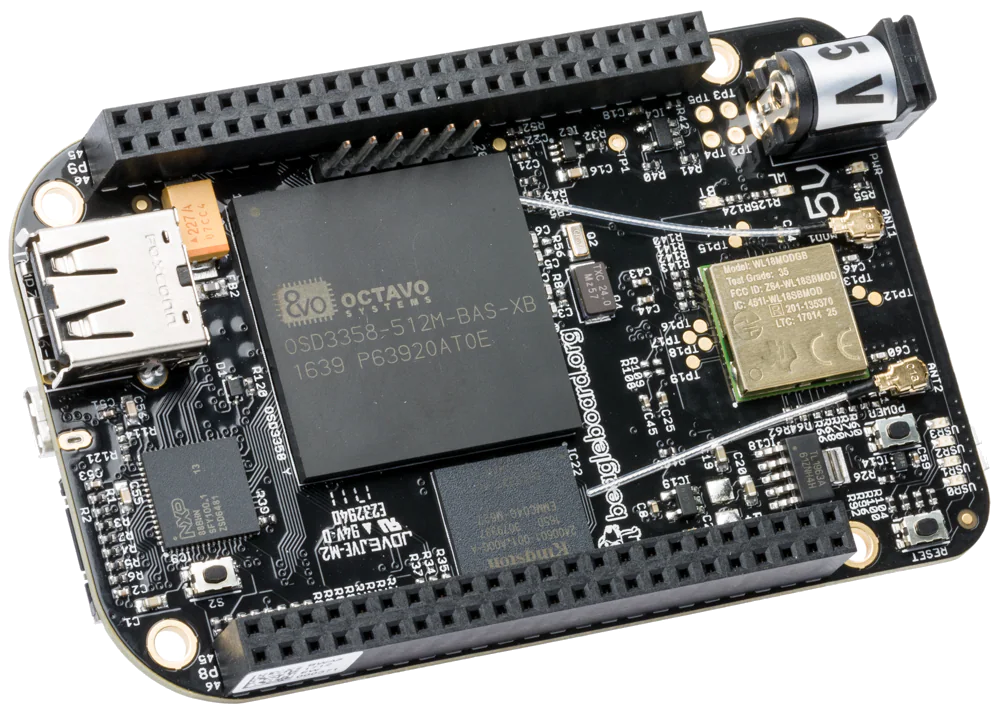
\includegraphics[height=5cm]{../slides/beagleboneblack-board/beagleboneblack.png}
  \end{center}
}

\feagendaonecolumn
{Labs}
{
  The practical labs of this training session use the following
  hardware peripherals to illustrate the development of Linux device
  drivers:

  \begin{itemize}
  \item A Wii Nunchuk, which is connected over the I2C bus to the
    BeagleBone Black board. Its driver will use the Linux {\em input}
    subsystem.
  \item An additional UART, which is memory-mapped, and will use the
    Linux {\em misc} subsystem.
  \end{itemize}

  While our explanations will be focused on specifically the Linux
  subsystems needed to implement these drivers, they will always be
  generic enough to convey the general design philosophy of the Linux
  kernel. The information learnt will therefore apply beyond just
  I2C, input or memory-mapped devices.
}


\section{Day 1 - Morning}

\feagendaonecolumn
{Lecture - Introduction to the Linux kernel}
{
  \begin{itemize}
  \item Kernel features
  \item Legal constraints with device drivers.
  \item Kernel user interface (/proc and /sys)
  \item User space device drivers
  \end{itemize}
}
\\
\feagendatwocolumn
{Lecture - Kernel sources}
{
  \begin{itemize}
  \item Specifics of Linux kernel development
  \item Coding standards
  \item Retrieving Linux kernel sources
  \item Tour of the Linux kernel sources
  \item Kernel source code browsers: cscope,
	Elixir Cross Referencer, VS Code...
  \end{itemize}
}
{Lab - Kernel sources}
{
  \begin{itemize}
  \item Making searches in the Linux kernel sources: looking for C
    definitions, for definitions of kernel configuration parameters,
    and for other kinds of information.
  \item Using the UNIX command line and then kernel source code
    browsers.
 \end{itemize}
}

\section{Day 1 - Afternoon}
\feagendatwocolumn
{Lecture - Configuring, compiling and booting the Linux kernel}
{
  \begin{itemize}
  \item Kernel configuration.
  \item Native and cross compilation. Generated files.
  \item Booting the kernel. Kernel booting parameters.
  \item Mounting a root filesystem on NFS.
  \end{itemize}
}
{Lab - Kernel configuration, cross-compiling and booting on NFS}
{
  {\em Using the BeagleBone Black board}
  \begin{itemize}
  \item Configuring, cross-compiling and booting a Linux kernel with
    NFS boot support.
  \end{itemize}
}
\\
\section{Day 2 - Morning}

\feagendatwocolumn
{Lecture - Linux kernel modules}
{
  \begin{itemize}
  \item Linux device drivers
  \item A simple module
  \item Programming constraints
  \item Loading, unloading modules
  \item Module dependencies
  \item Adding sources to the kernel tree
  \end{itemize}
}
{Lab - Writing modules}
{
  {\em Using the BeagleBone Black board}
  \begin{itemize}
  \item Write a kernel module with several capabilities.
  \item Access kernel internals from your module.
  \item Set up the environment to compile it
  \end{itemize}
}

\section{Day 2 - Afternoon}

\feagendatwocolumn
{Lecture - Linux device model}
{
  \begin{itemize}
  \item Understand how the kernel is designed to support device
    drivers
  \item The device model
  \item Binding devices and drivers
  \item Platform devices, Device Tree
  \item Interface in user space: \code{/sys}
  \end{itemize}
}
{Lab - Linux device model for an I2C driver}
{
  {\em Using the BeagleBone Black board}
  \begin{itemize}
  \item Implement a driver that registers as an I2C driver
  \item Modify the Device Tree to list an I2C device
  \item Get the driver called when the I2C device is enumerated at
    boot time
  \end{itemize}
}

\section{Day 3 - Morning}

\feagendatwocolumn
{Lecture - Introduction to the I2C API}
{
  \begin{itemize}
  \item The I2C subsystem of the kernel
  \item Details about the API provided to kernel drivers to interact
    with I2C devices
  \end{itemize}
}
{Lecture - Pin muxing}
{
  \begin{itemize}
  \item Understand the {\em pinctrl} framework of the kernel
  \item Understand how to configure the muxing of pins
  \end{itemize}
}

\feagendaonecolumn
{Lab - Communicate with the Nunchuk over I2C}
{
  {\em Using the BeagleBone Black board}
  \begin{itemize}
  \item Configure the pin muxing for the I2C bus used to communicate
    with the Nunchuk
  \item Extend the I2C driver started in the previous lab to
    communicate with the Nunchuk via I2C
  \end{itemize}
}

\section{Day 3 - Afternoon}

\feagendaonecolumn
{Lecture - Kernel frameworks}
{
  \begin{itemize}
  \item Block vs. character devices
  \item Interaction of user space applications with the kernel
  \item Details on character devices, \code{file_operations}, \code{ioctl()}, etc.
  \item Exchanging data to/from user space
  \item The principle of kernel frameworks
  \end{itemize}
}

\feagendatwocolumn
{Lecture - The input subsystem}
{
  \begin{itemize}
  \item Principle of the kernel {\em input} subsystem
  \item API offered to kernel drivers to expose input devices
    capabilities to user space applications
  \item User space API offered by the {\em input} subsystem
  \end{itemize}
}
{Lab - Expose the Nunchuk functionality to user space}
{
  {\em Using the BeagleBone Black board}
  \begin{itemize}
  \item Extend the Nunchuk driver to expose the Nunchuk features to
    user space applications, as a {\em input} device.
  \item Test the operation of the Nunchuk using \code{evtest}
  \end{itemize}
}

\section{Day 4 - Morning}

\feagendatwocolumn
{Lecture - Memory management}
{
  \begin{itemize}
  \item Linux: memory management - Physical and virtual (kernel and user) address spaces.
  \item Linux memory management implementation.
  \item Allocating with \code{kmalloc()}.
  \item Allocating by pages.
  \item Allocating with \code{vmalloc()}.
  \end{itemize}
}
{Lecture - I/O memory}
{
  \begin{itemize}
  \item I/O memory range registration.
  \item I/O memory access.
  \item Read / write memory barriers.
  \end{itemize}
}

\feagendaonecolumn
{Lab - Minimal platform driver and access to I/O memory}
{
  {\em Using the BeagleBone Black board}
  \begin{itemize}
  \item Implement a minimal platform driver
  \item Modify the Device Tree to instantiate the new serial port
    device.
  \item Reserve the I/O memory addresses used by the serial port.
  \item Read device registers and write data to them, to send
    characters on the serial port.
  \end{itemize}
}

\section{Day 4 - Afternoon}

\feagendatwocolumn
{Lecture - The misc kernel subsystem}
{
  \begin{itemize}
  \item What the {\em misc} kernel subsystem is useful for
  \item API of the {\em misc} kernel subsystem, both the kernel side
    and user space side
  \end{itemize}
}
{Lab - Output-only serial port driver}
{
  {\em Using the BeagleBone Black board}
  \begin{itemize}
  \item Extend the driver started in the previous lab by registering
    it into the {\em misc} subsystem
  \item Implement serial port output functionality through the {\em
      misc} subsystem
  \item Test serial output from user space
  \end{itemize}
}

\feagendatwocolumn
{Lecture - Processes, scheduling, sleeping and interrupts}
{
  \begin{itemize}
  \item Process management in the Linux kernel.
  \item The Linux kernel scheduler and how processes sleep.
  \item Interrupt handling in device drivers: interrupt handler
    registration and programming, scheduling deferred work.
  \end{itemize}
}
{Lab - Sleeping and handling interrupts in a device driver}
{
  {\em Using the BeagleBone Black board}
  \begin{itemize}
  \item Adding read capability to the character driver developed
    earlier.
  \item Register an interrupt handler.
  \item Waiting for data to be available in the \code{read()} file operation.
  \item Waking up the code when data is available from the device.
  \end{itemize}
}

\section{Day 5 - Morning}

\feagendatwocolumn
{Lecture - Locking}
{
  \begin{itemize}
  \item Issues with concurrent access to shared resources
  \item Locking primitives: mutexes, semaphores, spinlocks.
  \item Atomic operations.
  \item Typical locking issues.
  \item Using the lock validator to identify the sources of locking
    problems.
  \end{itemize}
}
{Lab - Locking}
{
  {\em Using the BeagleBone Black board}
  \begin{itemize}
  \item Add locking to the current driver
  \end{itemize}
}

\feagendatwocolumn
{Lecture - Driver debugging techniques}
{
  \begin{itemize}
  \item Debugging with printing functions
  \item Using Debugfs
  \item Analyzing a kernel oops
  \item Using kgdb, a kernel debugger
  \item Using the Magic SysRq commands
  \end{itemize}
}
{Lab - Investigating kernel faults}
{
  {\em Using the BeagleBone Black board}
  \begin{itemize}
  \item Studying a broken driver.
  \item Analyzing a kernel fault message and locating the problem in the
    source code.
  \end{itemize}
}

\section{Day 5 - Afternoon}

\feagendatwocolumn
{Lecture - ARM board support and SoC support}
{
  \begin{itemize}
  \item Understand the organization of the ARM support code
  \item Understand how the kernel can be ported to a new hardware
    board
  \end{itemize}
}
{Lecture - Power management}
{
  \begin{itemize}
  \item Overview of the power management features of the kernel
  \item Topics covered: clocks, suspend and resume, dynamic frequency
    scaling, saving power during idle, runtime power management,
    regulators, etc.
  \end{itemize}
}

\feagendaonecolumn
{Lecture - The Linux kernel development process}
{
  \begin{itemize}
  \item Organization of the kernel community
  \item The release schedule and process: release candidates, stable
    releases, long-term support, etc.
  \item Legal aspects, licensing.
  \item How to submit patches to contribute code to the community.
  \item Kernel resources: books, websites, conferences
  \end{itemize}
}

\feagendatwocolumn
{Lecture - If time left}
{
  \begin{itemize}
  \item DMA
  \item mmap
  \end{itemize}
}
{Questions and Answers}
{
  \begin{itemize}
  \item Questions and answers with the audience about the course topics
  \item Extra presentations if time is left, according what most
        participants are interested in.
  \end{itemize}
}

\end{document}

